\documentclass[border=4pt]{standalone}
\usepackage[T1]{fontenc}
\usepackage{tikz}
\usetikzlibrary{arrows.meta,positioning,fit,backgrounds,shapes.geometric,calc}
\definecolor{orch}{HTML}{234767}
\definecolor{ctx}{HTML}{EAF1F8}
\definecolor{retr}{HTML}{E2F0ED}
\definecolor{ext}{HTML}{F7EBDD}
\definecolor{infra}{HTML}{F1F3F5}
\tikzset{
 every node/.style={font=\sffamily\fontsize{8.5}{10}\selectfont,align=center},
 block/.style={draw=orch!80,fill=white,rounded corners=1.5pt,minimum height=7mm,inner sep=3pt,line width=.55pt},
 context/.style={block,fill=ctx},
 engine/.style={block,fill=orch,text=white},
 retrieval/.style={block,fill=retr},
 external/.style={block,fill=ext},
 storage/.style={block,fill=infra},
 flow/.style={-{Stealth[length=2mm]},draw=orch!90,line width=.65pt},
 control/.style={flow,dashed},
 error/.style={flow,densely dotted},
 group/.style={draw=orch!50,rounded corners=3pt,inner sep=5pt,line width=.5pt},
 heading/.style={font=\sffamily\bfseries\fontsize{8.5}{10}\selectfont,text=orch},
 edgelabel/.style={font=\sffamily\fontsize{7.5}{9}\selectfont,fill=white,inner sep=1pt,text=orch}
}

\begin{document}
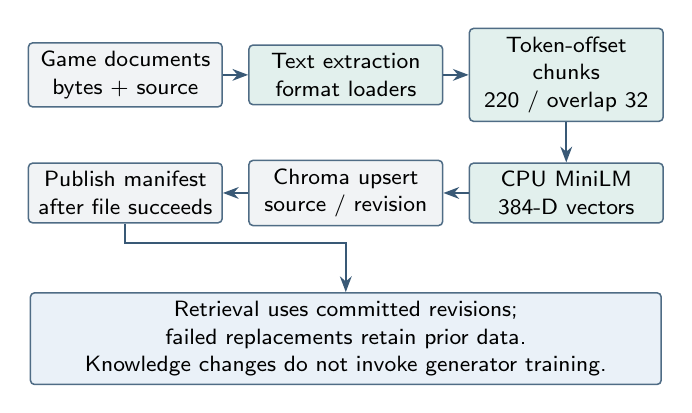
\begin{tikzpicture}
\node[storage,text width=2.25cm] (docs) at (0,0) {Game documents\\bytes + source};
\node[retrieval,text width=2.25cm] (extract) at (2.8,0) {Text extraction\\format loaders};
\node[retrieval,text width=2.25cm] (chunk) at (5.6,0) {Token-offset chunks\\220 / overlap 32};
\node[retrieval,text width=2.25cm] (embed) at (5.6,-1.5) {CPU MiniLM\\384-D vectors};
\node[storage,text width=2.25cm] (store) at (2.8,-1.5) {Chroma upsert\\source / revision};
\node[storage,text width=2.25cm] (manifest) at (0,-1.5) {Publish manifest\\after file succeeds};
\node[context,text width=7.8cm] (ready) at (2.8,-3.35) {Retrieval uses committed revisions; failed replacements retain prior data.\\Knowledge changes do not invoke generator training.};
\draw[flow] (docs) -- (extract);
\draw[flow] (extract) -- (chunk);
\draw[flow] (chunk) -- (embed);
\draw[flow] (embed) -- (store);
\draw[flow] (store) -- (manifest);
\draw[flow] (manifest.south) -- ++(0,-.25) -| (ready.north);
\end{tikzpicture}
\end{document}
